\chapter{测试与实验}

\section{测试总述}
本章节包含了对本文所带的样例实现进行简单测试的过程和结果。测试主要通过对客户端库进行数个集成的测试,而服务端不包含单独的测试。对服务端的测试被包含在对客户端库的测试中,通过对网络通信函数的测试来间接完成。对每个测试本章节亦会给出其对应的基准测试结果。

\section{测试环境描述}

\subsection{系统环境}

\begin{itemize}
    \item 操作系统:Arch Linux(Rolling)\footnote{即滚动性发行,所有软件包总是上游最新的}
    \item Golang 工具链:版本 1.20.4,Arch 软件包仓库版本 \verb|go 2:1.20.4-1|
    \item 处理器:AMD Ryzen 9 4900HS with Radeon Graphics (16) @ 3.000GHz
\end{itemize}

\subsection{样例实现使用的第三方库}

以下为本方案所使用的第三方库列表。其中,\verb|github.com/tuneinsight/lattigo/v4| 为本方案的核心库,其余为辅助库。

\begin{minted}{go}
require (
    github.com/tuneinsight/lattigo/v4 v4.1.0
    github.com/urfave/cli/v2 v2.25.1

    github.com/google/uuid v1.3.0
    github.com/kr/pretty v0.3.1
    github.com/mattn/go-sqlite3 v1.14.16
    github.com/pkg/errors v0.9.1
)
\end{minted}

\section{测试样例描述}

本方案编写了如下测试函数,其中每个测试函数都有对应的性能基准测试函数:

\begin{itemize}
    \item \verb|func TestCKKSEncryptAndDecrypt(*testing.T)|:对本文代码封装的 CKKS 加密和解密函数进行正确性测试;
    \item \verb|func TestTransferBySenderPK(*testing.T)|:测试能否正确生成交易;
    \item \verb|func TestTransferByReceiptPK(*testing.T)|:同上;
    \item \verb|func TestAcceptTransactionByTransaction(*testing.T)|:测试能否正确生成确认消息;
    \item \verb|func TestRegisterUser(*testing.T)|:测试生成密钥对,将用户信息提交给服务端的功能,并且测试服务端是否能够正确地将用户信息存储到数据库中而不报出异常;
    \item \verb|func TestRegisterSwk(*testing.T)|:在上述函数基础上,测试生成交换密钥,并将其提交给服务端;
    \item \verb|func TestCreateTransferJobBySenderPK(*testing.T)|:在上述函数基础上,测试能否正确向服务端提交交易信息,以及服务端是否会正确响应请求;
    \item \verb|func TestCreateTransferJobByReceiptPK(*testing.T)|:同上,但是测试的是以收款方公钥加密的密文发起的交易,涉及了双方签名和确认的过程,总共两次网络交互;
    \item \verb|func BenchmarkReEncryptCTWithSwk(*testing.B)|:对重加密性能进行评估的基准测试函数
\end{itemize}

以及以下的辅助函数:

\begin{itemize}
    \item \verb|func initTestRandomUser()|:准备单次测试环境,包括全局变量等。
    \item \verb|func makeNewRandomUser(string)|:生成随机用户。
\end{itemize}

\section{实验和基准测试结果}

本文在测试时,使用下述命令,调用 Golang 工具链提供测试功能,对方案进行功能测试和性能测试。

\begin{minted}{shell}
$ go run ./cmd/server # 使服务端上线

# 进行集成测试
$ /usr/bin/go test -timeout 30s \
  -coverprofile=/tmp/vscode-goUzLyPD/go-code-cover \
  github.com/CamberLoid/Chimata/internal/clientlib

# 进行基准性能测试
$ /usr/bin/go test -benchmem -run=^$ \
  -coverprofile=/tmp/vscode-goUzLyPD/go-code-cover \
  -bench . github.com/CamberLoid/Chimata/internal/clientlib

$ /usr/bin/go test -benchmem -run=^$ \
  -coverprofile=/tmp/vscode-goUzLyPD/go-code-cover \
  -bench . github.com/CamberLoid/Chimata/internal/serverlib
\end{minted}

以 VSCode 的 Golang 插件,执行的测试结果如下图\ref{Fig:test} \ref{Fig:benchmark}所示。 

\begin{figure}[h]
    \centering
    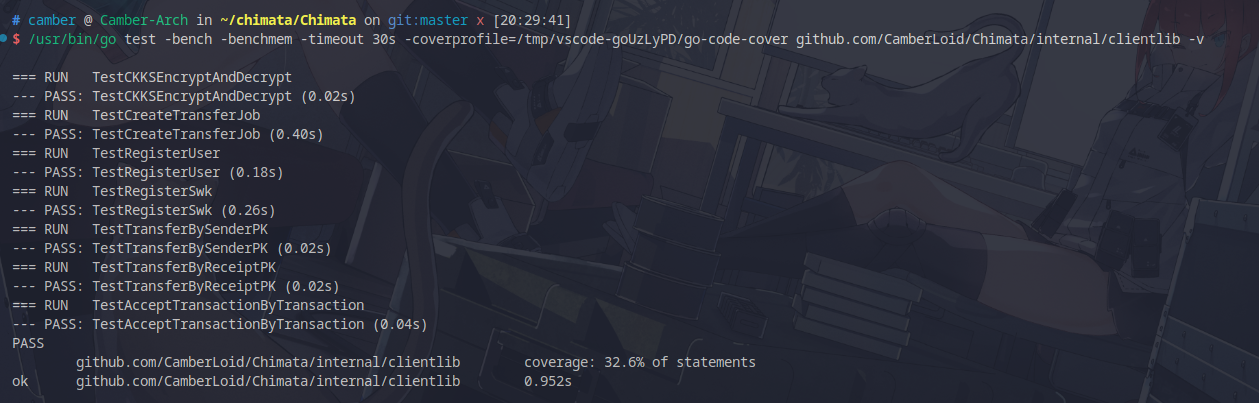
\includegraphics[width=0.9\linewidth]{./Figures/Test.png}
    \caption{以默认参数执行的集成测试输出}\label{Fig:test}
\end{figure}

\begin{figure}
    \centering
    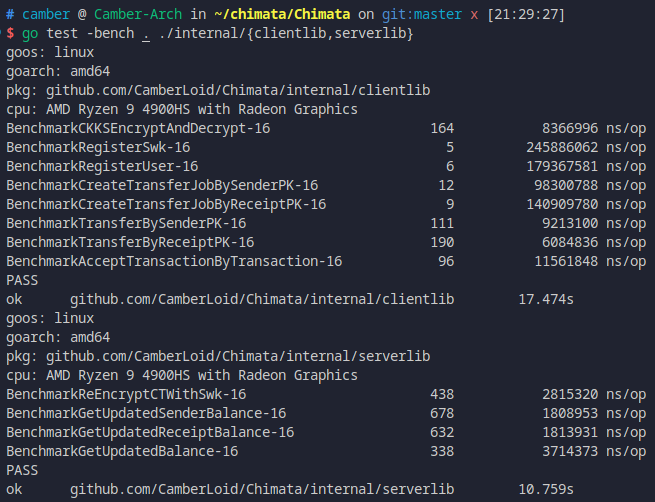
\includegraphics[width=0.9\linewidth]{./Figures/Bench_Overall.png}
    \caption{以默认参数执行的性能测试输出}\label{Fig:benchmark}
\end{figure}


在网络交互部分,笔者对 \verb|TestTransferBySenderPK| 和 \\
\verb|TestTransferByReceiptPK| 进行了基准测试,测试内容为连续运行 100 次各方法,每次均和服务器交互,生成一笔交易并进行确认。测试结果如图\ref{Fig:bench_transaction}所示。可以注意到,服务端处理一次以转出方公钥加密密文的交易,平均耗时约 115 毫秒;而处理一次以转入方公钥加密的密文发起的交易,涉及到创建和确认两步,平均耗时约 140 毫秒。测试后的数据库大小约为 57 MB,如图\ref{Fig:database_size}所示,平均每笔交易占用约 290 KB 的存储空间\footnote{未考虑用户信息的存储消耗},即每 1 GB 存储空间可以容纳约 3627 笔交易。图\ref{Fig:server}显示了服务端处理方法 \verb|/transaction/create/byReceiptPK| 的输出。

\begin{figure}
    \centering
    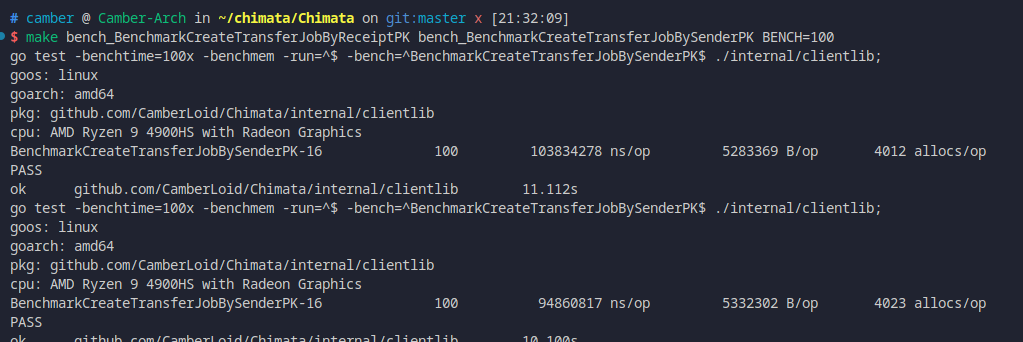
\includegraphics[width=0.8\linewidth]{./Figures/Bench_Transaction_all.png}
    \caption{交易基准测试数据}\label{Fig:bench_transaction}
\end{figure}

\begin{figure}
    \centering
    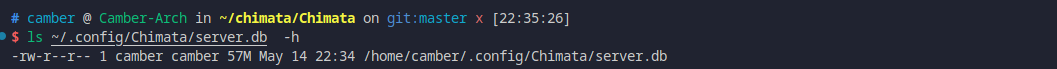
\includegraphics[width=0.8\linewidth]{./Figures/Test_Database_Size.png}
    \caption{数据库大小}\label{Fig:database_size}
\end{figure}

\begin{figure}
    \centering
    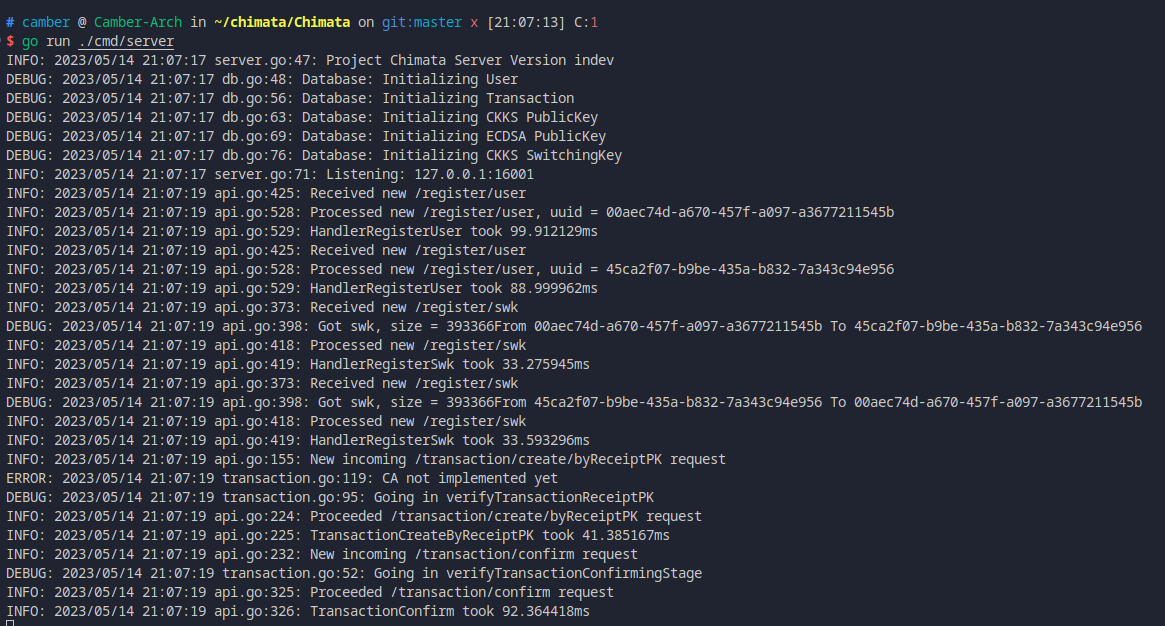
\includegraphics[width=0.8\linewidth]{./Figures/Server_ReceiptPK.png}
    \caption{服务端日志输出}\label{Fig:server}
\end{figure}


在涉及网络交互的部分之外,本文也对加解密性能和重加密性能进行测试。测试结果如图\ref{Fig:benchmark}和图\ref{Fig:bench_reencrypt}所示,平均每次加解密时间总和约为 12 ms,而重加密的时间开销约为 3 ms。可以看到,加解密性能和重加密性能都较为优秀。与网络交互部分的实验数据进行对比可以发现,实际密码学函数的开销,即加解密和重加密的时间的总和,约占据了单次网络交互时间的约 15\% 的比例。可以推测,在网络交互部分,服务端的数据库操作开销占比较大。

\begin{figure}[h]
    \centering
    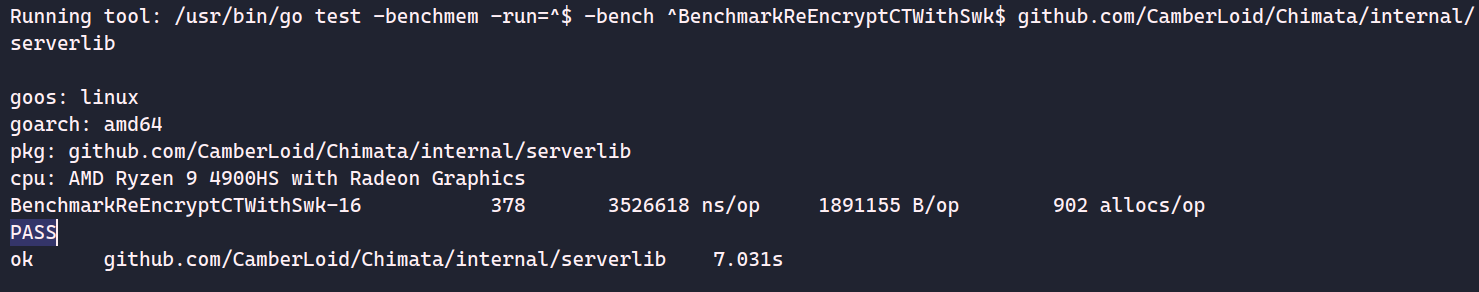
\includegraphics[width=0.8\linewidth]{./Figures/Bench_ReEncrypt.png}
    \caption{密文重加密的基准测试数据}\label{Fig:bench_reencrypt}
\end{figure}

\pagebreak

\pagebreak

\section{本章小结}

为测试提出方案的性能,本章对基于同态加密的用户交易金额隐私保护交易方案中的密码学部分以及交易处理部分,借助 Golang 工具链进行了基准测试。实验结果表明,在预设的安全参数下,本文所提出的交易方案,在密码学部分具有较高的效率;从总体来看,本方案的单次交易性能也符合预期,在实际应用中具有高效性。
